\documentclass{beamer}
\usetheme{default}

\usepackage{graphicx}
\graphicspath{{../../images/}}

\setbeamertemplate{caption}[numbered]

\title{Chapter-13: Arsitektur Continer}
\subtitle{IF231303-Software Architecture\\Pradita University}
\author{Richwen Canady, Desfantio Wuidjaja, Vincenzo Matalino}
\begin{document}
	
	\begin{frame}[plain]
		\maketitle
	\end{frame}
	
	\begin{frame}{Container}
		\begin{figure}[h]
			\centering
			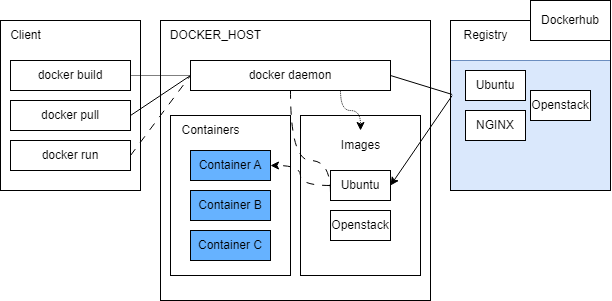
\includegraphics[width=\textwidth]{DockerDiagram.png}
			\caption{Diagram Docker.}
			\label{fig:ContainerDiagram}
		\end{figure}
	\end{frame}
	
	\begin{frame}{Latar Belakang}
                \item Konsep container berasal dari teknologi chroot pada sistem operasi UNIX. Teknologi ini memungkinkan pengguna untuk membuat lingkungan kerja yang terisolasi pada sistem operasi UNIX.
                \item Namun, teknologi chroot memiliki beberapa keterbatasan, seperti pengguna harus mengkonfigurasi secara manual, tidak mendukung manajemen sumber daya.
                \item Pada tahun 2008, LXC (Linux Containers) mengembangkan teknologi container sebagai solusi untuk mengatasi keterbatasan teknologi chroot pada sistem operasi UNIX.
                \item Pada tahun 2013, Docker dirilis sebagai implementasi teknologi container yang lebih ramah pengguna dan mudah digunakan.
	\end{frame}

        \begin{frame}{Pengertian}
		\begin{itemize}
			\item Container Architecture
                \\Sebuah konsep arsitektur yang dirancang untuk menjalankan aplikasi dalam container.
                \item Container
                \\Metode menjalankan aplikasi yang memungkinkannya berjalan secara konsisten di berbagai lingkungan komputasi.
                \item Docker
                \\Platform open source untuk mengembangkan, menguji, dan mengimplementasikan aplikasi dalam container. 
		\end{itemize}
	\end{frame}
	
	\begin{frame}{Kelebihan}
		Kelebihan dari menggunakan docker dalam pembuatan aplikasi adalah:
		\begin{itemize}
			\item Docker mempunyai konfigurasi yang sederhana, sehingga dapat disesuaikan dengan kebutuhan aplikasi yang dikembangkan pengguna.
			\item Docker mempunyai tingkat keamanan yang baik.
			\item Docker dapat dijalankan pada beberapa platform \textit{Cloud}, sehingga pengguna dapat melakukan porting aplikasi dengan lebih mudah dan fleksibel.
			\item Docker mempunyai ukuran yang cukup ringan, dan lebih hemat sumber daya.
			\item Docker memiliki fitur \textit{debugging}.
			
		\end{itemize}
	\end{frame}
	
	\begin{frame}{Kekurangan}
		Kekurangan dari menggunakan docker dalam pembuatan aplikasi adalah:
		\begin{itemize}
			\item Docker tidak menyediakan opsi penyimpanan, sehingga data yang disimpan di dalam sebuah container masih perlu di-\textit{back up} secara manual.
			\item \textit{Cross-platform compatibility} docker kurang fleksibel.
			\item Terdapat banyak fitur yang tidak disediakan oleh docker, sehingga pengguna harus meng-\textit{install} perangkat lunak eksternal untuk menggantikannya.
		\end{itemize}
	\end{frame}
	
	\begin{frame}{Perbedaan}
		Terdapat beberapa perbedaan antara \textit{container architecture} dan \textit{virtualization} yaitu:
		\begin{itemize}
			\item Isolasi
			\item Sistem Operasi
			\item Portabilitas
			\item \textit{Overhead}
			\item Orkestrasi
		\end{itemize}
	\end{frame}

 	\begin{frame}{Perbedaan}
            \begin{figure}[h]
                \centering
	        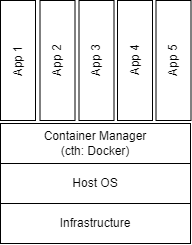
\includegraphics[width=.35\textwidth]{ContainerDiagram.png}
	        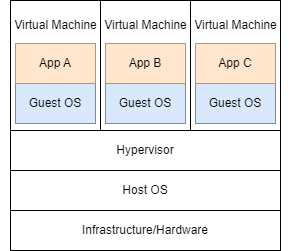
\includegraphics[width=.5\textwidth]{VirtualizationDiagram.png}
	        \caption{Arsitektur Container vs Virtualization.}
	        \label{fig:ContainerDiagram}
	    \end{figure}
	\end{frame}

	\begin{frame}{Contoh Kasus}
            \item Terdapat sebuah aplikasi php yang sudah di-\textit{develop} menggunakan php7. Belum tentu aplikasi tersebut bisa dijalankan di komputer lain yang menjalankan php5.
            \item Dengan menggunakan docker, meskipun pada dasarnya komputernya menggunakan php5, \textit{image} dan \textit{container}nya sudah ada php7 jadinya tidak perlu konfigurasi ulang.
	\end{frame}

\end{document}
